% !TEX root = ../paper.tex
%http://sphweb.bumc.bu.edu/otlt/MPH-Modules/BS/BS704_HypothesisTesting-ANOVA/BS704_HypothesisTesting-Anova_print.html
\section{Results}\label{sec:results}
The following section presents the results that were gathered throughout the experiment.
Here we aim to uncover what variables in our studies were of significance. 
Some data points needed to be removed from the experiments, in order to gain a clearer understanding of the experimental outcomes. 

For the \target, we started with a total of 7344 attempts.
176 were removed because of system errors, where the system wrongly activated a technique attempt even though the user did not intend to do so.
Another 406 attempts were removed as outliers using the Outlier Labeling method described by Hoaglin and Iglewicz in Resistant Rules for Outlier Labeling \cite{Hoaglin:1987}.
This gave us a total of 6762 attempts for the first study.

For the \accuracy, we started with a total of 4752 attempts.
111 attempts were removed due to system errors. 
Another 138 attempts were removed with the same Outlier Labeling method used above.
This gave us a total of 4503 attempts for the second study.

\Cref{tab:numberOfAttempts} shows the final number of attempts each technique had in the two different studies.

\begin{table}[H]
	\centering
	\begin{adjustbox}{width=\columnwidth}
		{
			\def\arraystretch{1.5}
			\begin{tabular}{c c c c c}
				& \multicolumn{4}{c}{\textbf{STUDY ONE}} \\
				\cline{2-5}
				& \textbf{Grab} & \textbf{Swipe} & \textbf{Throw} & \textbf{Tilt} \\ \hline
				\textbf{Push} & 830 & 835 & 814 & 862 \\ \hline
				\textbf{Pull} & 784 & 893 & 867 & 877 \\ \hline
			\end{tabular}
		}
		{
			\def\arraystretch{1.5}
			\begin{tabular}{c c c c c}
				& \multicolumn{4}{c}{\textbf{STUDY TWO}} \\
				\cline{2-5}
				& \textbf{Grab} & \textbf{Swipe} & \textbf{Throw} & \textbf{Tilt} \\ \hline
				\textbf{Push} & 551 & 576 & 561 & 582 \\ \hline
				\textbf{Pull} & 533 & 576 & 569 & 555 \\ \hline
			\end{tabular}
		}
	\end{adjustbox}
	\caption{Number of attempts for each technique in each study}
	\label{tab:numberOfAttempts}
\end{table}

\subsection{STUDY ONE: Success rate}
Here we present results relating to whether or not the user was successful in hit the target, which we will be referring to as effectiveness when discussing the results in the \target. 

To see whether or not each technique had an association with the success rate of each attempt, and was not just noise, we performed a Pearsons Chi-Square test.
For the \push techniques, $\chi^2(3)=121.950$, $p<0.001$, and for the \pull techniques we got $\chi^2(3)=438.473$, $p<0.001$. 
This means that both \push and \pull techniques had an association with the success rate of each attempt.
\Cref{tab:successRate} shows the success rate for each of the techniques. 

\begin{table}[H]
	\centering
	\def\arraystretch{1.5}
		\begin{tabular}{c c c c c}
			& \multicolumn{4}{c}{\textbf{Hit Success Means}} \\
			\cline{2-5}
			& \textbf{Grab} & \textbf{Swipe} & \textbf{Throw} & \textbf{Tilt} \\ \hline
			\textbf{Push} & 95.9\% & 96\% & 93.2\% & 83.3\% \\ \hline
			\textbf{Pull} & 94\% & 97.5\% & 96.7\% & 71.8\% \\ \hline
		\end{tabular}
	\caption{Success rate for each technique in \target}
	\label{tab:successRate}
\end{table}

We then looked at each technique individually to see where the association may be.
Our post-hoc tests show that the \throw \push technique did not have a significant association ($p=0.55$) with the success rate of each attempt.
All other techniques had a significant association ($p<0.004$) with the success rate of each attempt. 

\subsection{STUDY ONE: Time taken}
Here, we present results in regards to how long each user took in performing each technique in the \target. 
When discussing these results, we will be referring to a technique's efficiency.

We performed a linear mixed effects model analysis on the data to see how time was affected by the different aspects of our experiment. 
We found that neither \effectiveness nor \direction had an effect on the time each user took per attempt. 
However, the \targetsize ($F_{1,6695.228} = 91.634, p < 0.001$) and the \technique ($F_{1,6695.228} = 91.634, p < 0.001$) did have significant effects on the time taken. 
We performed a post-hoc LSD pairwise comparison to see how each technique differed from one another and found that all techniques were significantly different $(p<0.001)$ from each other. 

We also found that there were other interactions between the variables that were affecting the time for each attempt differently. 
$Direction \times Technique$  ($F_{3,6694.657} = 52.272, p < 0.001$), $Effectiveness \times Technique$  ($F_{3,6696.169} = 5.227, p < 0.001$) and finally $Effectiveness \times Direction \times Technique$  ($F_{3,6696.038} = 10.235, p < 0.001$) all showed to be significant interactions. 
A post-hoc LSD pairwise comparison on \direction and \technique showed that for each technique the difference in time between \push and \pull were significant.
We then did a post-hoc LSD pairwise comparison on \effectiveness for each \technique and \direction to see where that significance was and the only significantly different pair was between a successful and unsuccessful attempt of the \grab \pull technique $(p < 0.001)$ meaning that an unsuccessful \grab \pull takes a significantly longer time to perform than a successful \grab \pull.

\Cref{tab:efficiency} and \Cref{fig:efficiencyGraph} shows the mean time taken for each technique and direction.

\begin{table}[H]
	\centering
	\def\arraystretch{1}
		\begin{tabular}{c c c c c}
			& \multicolumn{4}{c}{\textbf{Efficiency Means}} \B \\
			\cline{2-5}
			& \textbf{Grab} & \textbf{Swipe} & \textbf{Throw} & \textbf{Tilt} \T\B \\ \hline
			\textbf{Push} & 5.05 & 3.9 & 4.68 & 5.06 \T \\ 
			& (1.39) & (0.98) & (1.11) & (1.79) \B \\ \hline
			\textbf{Pull} & 5.74 & 3.67 & 4.12 & 4.55 \T \\ 
			& (1.57) & (0.86) & (1.01) & (1.61) \B \\ \hline
		\end{tabular}
	\caption{Efficiency means and (standard deviation) in seconds for each technique in \target.}
	\label{tab:efficiency}
\end{table}

\begin{figure}[H]{
	\centering
	\textbf{Efficiency}\\[4pt]
	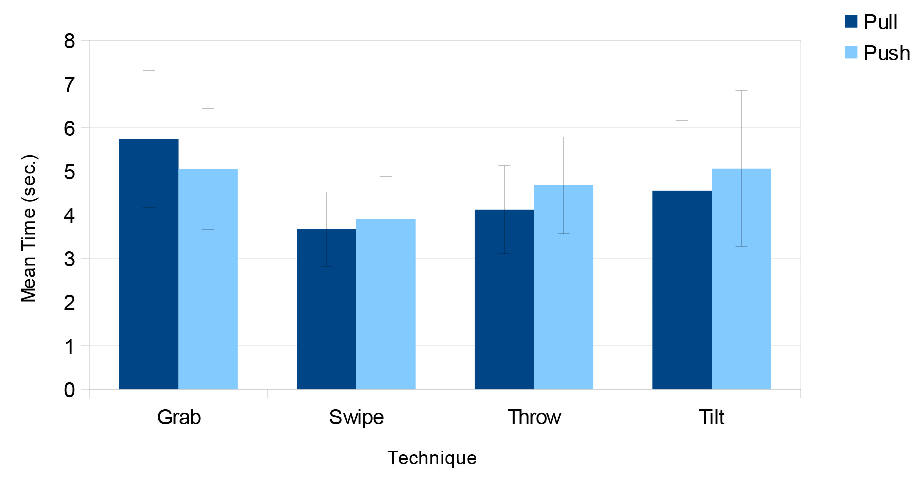
\includegraphics[width = 1\columnwidth ]{images/time_graph.pdf}} 
	\caption{
		Mean and standard deviation (seconds) for each technique in regards to efficiency.
	}
	\label{fig:efficiencyGraph}
\end{figure}

\subsection{STUDY TWO: Distance from target}
Here we present the results in regards to how far away from the center of the target (in pixels) each user was when performing the technique in the \accuracy. 
This is referred to as a techniques accuracy when we discuss the results. 

We performed a linear mixed effects model analysis on the data to see if each technique had a significant effect on the accuracy of each attempt. 

We found that \technique ($F_{3,4458.26}=193.869, p<0.001$) and \targetsize ($F_{1,4462.203}=100.016, p<0.001$) had an effect on accuracy, but the \direction of each technique did not have an effect on accuracy. 
We then performed a post-hoc LSD pairwise comparison to see were the differences lay, and found that all techniques were significantly different from each other ($p<0.003$ for all).

We also found that the $Direction \times Technique$ interaction had a significant effect on the accuracy ($F_{3,4457.354}=8.882, p<0.001$).
We then performed another LSD pairwise comparison between \technique for each \direction. 
We found that the only pair that was not significantly different from each other was between the techniques \grab \push and \throw \push ($p=0.508$). 
All others were significantly different from one another ($p<0.004$). 
Lastly, we did a LSD pairwise comparison between \direction for each \technique and the only pair not significantly different from each other were \grab \push and \grab \pull ($p=0.355$).
The difference between \pull and \push for all other techniques were significant ($p<0.044$).

\begin{table}[H]
	\centering
	\def\arraystretch{1}
		\begin{tabular}{c c c c c}
			& \multicolumn{4}{c}{\textbf{Accuracy Means}} \B \\
			\cline{2-5}
			& \textbf{Grab} & \textbf{Swipe} & \textbf{Throw} & \textbf{Tilt} \T\B \\ \hline
			\textbf{Push} & 16.8 & 14.14 & 16.24 & 28.03 \T \\ 
			& (10.5) & (9.32) & (10.29) & (19.7) \B \\ \hline
			\textbf{Pull} & 17.65 & 12.4 & 15.07 & 32.71 \T \\
			& (10.92) & (8.59) & (10.25) & (21.49) \B \\ \hline
		\end{tabular}
	\caption{Accuracy means and (standard deviation) in pixels for each technique in \accuracy.}
	\label{tab:accuracy}
\end{table}

\Cref{tab:accuracy} and \Cref{fig:accuracyGraph} shows the mean distance from the center for each technique and direction.
\begin{figure}[H]{
	\centering
	\textbf{Accuracy}\\[4pt]
	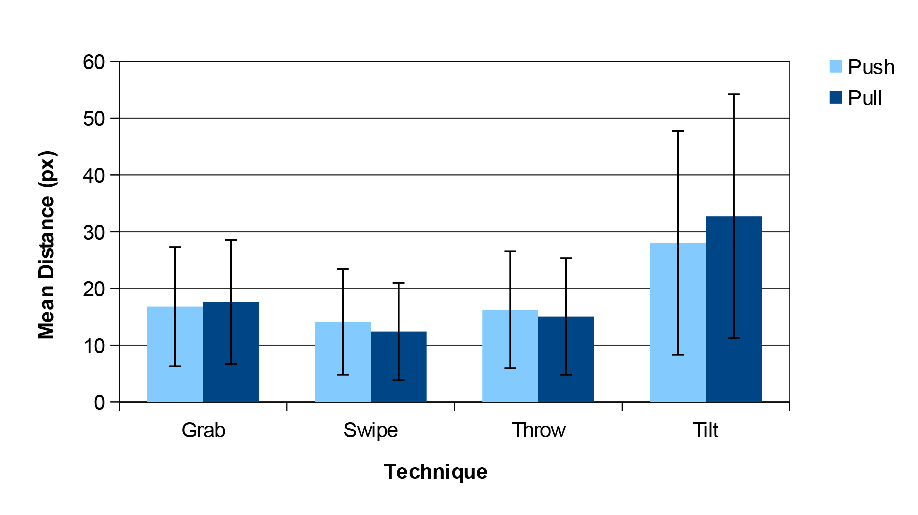
\includegraphics[width = 1\columnwidth ]{images/distance_graph.pdf}} 
	\caption{
		Mean and standard deviation (pixel) for each technique in regards to accuracy.
	}
	\label{fig:accuracyGraph}
\end{figure}